\chapter{Results}

For the project, three main goals were established. The usability of the level editor was to
be improved to make the system easier to work with. The level generator needed to be
augmented to better suit and interactive system, while being configurable and providing a
greater amount of variety in the generated levels. Collaborative elements to level creation
were to be added to support designers while creating levels.

The usability of the system was greatly improved compared to its previous iteration. The
efficiency and feedback of the editor received the most attention. Efficiency was improved
by adding bulk operations that are commmon to many other direct manipulation interfaces. A
bulk select was added, which supports the "re-generate", "delete", and "add chunk" 
operations. Through the use of the chunk library, the user can create patterns of level 
segments that can be paster into the level directly, speeding up repetitive work. More
experienced users shold be able to accelerate the level creation process by generating
ideas. Additionally, accelerators for common actions like "save", "save as", "open" and
"undo" were added. Feedback was provided for the actual design task itself. Whenever a
change is made to a level, the user can immediately check whether or not it is playable, and
correct mistakes. Elements in the interface such as the "Level Overview" panel provide the 
user with extra information that can be used to adjust the level, but are more passive
that the playability message, and have to be interpreted by the user. Novice and advanced
users can save time, which can instead be spent on level design. Some improvements could
be made to the editor to account for visibility are learnability issues. For example,
generating a level takes a few seconds on a fast machine, but the application appears to
"freeze" while this happens. A loading icon or some progress bar would be better suited to
indicating progress. The user also needs experience with the algorithm, or will probably
be confused, since no tutorial or documentation about it is available through the
software.

In terms of functionality as a level editor defined by Rouse, these requirements were met.
As the suer edits the level, a complete representation of how the final level looks is
provided. The editor provides the user with extra information about the level, including
playability, the distribution of enemies and components, and the behaviour of each tile. 
Levels can instantaneously be playtested from a single button. The user is also able to 
test from any position, to avoid having to replay large level sections. The editor also 
succeeds in allowing the user the power to change gameplay critical parts of the level. 
Users may resize the level, move the exit, place any tile, any enemy they want, so user
freedom is not an issue.

The level generationj algorithm created is configurable. Through the use of the canvas
and system dialogs, the user is able to add content that the generator can use to create
levels. The speed of the generator is also reasonable. On both a lpatiop with a low-end
processor and a high-end desktop, a 256x15 level is generated in under 10 seconds, which
makes the generator available as a choice in real-time games. To contrast, ORE generates
its levels in 15 seoncds with a chunk library of size 40.

In order to evaluate the results of mORE in terms of producing sufficiently varied levels,
a comparison against the default InfiniteTux generator, the Notch generator was made. In the
project proposal, the expressivity of the level generator was to be evaluated by its 
expressive range, as described by the leniency and linearity characteristics, similar to
Smith's evaluation of Tanagra in \cite{smith2010}. Linearity measures how well a straight
line fits to the level geometry, in a similar way to how a straight line is fit to a set of
observations in statistics. Leniency measures the amount of risk in a level, and assigns
scores to a level by how likely the player is to lose based on the presence of obstacles.
Measuring leniency means finding gaps and dynamic obstalces in a level. In Tanagra's case,
it is straightforward because Tanagra understands the context that it places these
obstacles in, but mORE does not have the same context, and cannot determine where obstacles
exist without some post-processing step. Therefore, the expressive range of mORE was not
measured, and another metric for level variability was chosen.

Lucas and Volz created an approach for analysin the amount of variability between two levels
\cite{lucas2019}, coined Kullback-Leibler Divergence (KL Divergence). KL Divergence works by
counting all  occurrences of patterns of some size in a level by convolving over its tiles.
The count is then used to create a probability distribution. Two levels are "the same"
if the KL Divergence of their probability distributions is equal to 0. Otherwise, the more
positive the KL-Divergence is, the more varied the levels are.

For each level genertor, 10,000 pairs or levels were created. For each, the KL Divergence
was calculated, which produced a probability distribution of KL Divergence for the
Notch and mORE generators. The process was repeated three times, using 2x2, 4x4, and 6x6
patterns. Descriptive statistics for each distribution at each feature size are provided
in \autoref{table:more-ore-desc}. To show that mORE leVels are more varied than Notch
generator levels, a one-tailed t-test was performed for the distributions of each pattern
size. p should be less than 0.05 for the results to be significant, and to be able to
reject the null hypopthesis that $\mu_1$, the sample mean of mORE's level variability, is less
than or equal to $\mu_2$, the sample mean of Notch's level variability. The results of these
three tests are shown in \autoref{table:t-test}, and graphically summarised in 
\autoref{fig:boxplot}. 

For each feature size, the KL Divergence distributions are compared between the Notch and 
mORE generators. For features 2x2 and 6x6 in size, p is less than 0.05, so the mORE
generator does produce more varied levels for these feature sizes. For feature size 4x4,
the p-value is not less than 0.05, so the null hypothesis cannot be rejected. In terms of
level variability, the mORE generator does produce more vaired levels with the chunk library
described in \autoref{fig:chunk-library} than the Notch generator. For 4x4 patterns, it could
not be shown that the mORE generator produces more varied levels at this feature size,
For 6x6 features, the p-value is much less than 0.05, so the distribution of 6x6 features
differes significantly between the two generators. These results show that in some cases,
the mORE generator produces more varield levels than the Notch generator, so in this regard
it is successful. With a different chunk library, it seems plausible to claim that mORE could
produce significantly more varied results for 4x4 features. Another statistic worth 
mentioning is that the distribution for mORE are more speard out than every distribution for
the Notch generator. The maximum values are significantly higher than Notch's generator, and
the minimum values are slightly lower. Therefore, in a limited number of cases, mORE was 
able to produce a pair of levels that differ substantially from one another.

\begin{table}[ht]
\begin{tabular}{| c | c | c | c | c |}\hline
Generator and feature size & Min & $Q_1$ & Median & Mean \\\hline
Notch 2x2 & 1.779 & 7.220 & 8.982 & 9.431 \\\hline
mORE 2x2 & -2.502 & 4.830 & 7.276 & 9.768 \\\hline
Notch 4x4 & 9.778 & 12.507 & 13.253 & 13.394 \\\hline
mORE 4x4 & 6.431 & 10.211 & 11.419 & 12.282 \\\hline
Notch 6x6 & 11.990 & 13.950 & 14.450 & 14.540 \\\hline
mORE 6x6 & 10.210 & 14.080 & 15.030 & 15.510 \\\hline
\end{tabular}


\begin{tabular}{| c | c | c | c |}\hline
Generator and feature size & $Q_3$ & Max & \emph{s} \\\hline
Notch 2x2 & 11.138 & 39.885 & 3.213\\\hline
mORE 2x2 & 10.641 & 344.329 & 14.680\\\hline
Notch 4x4 & 14.110 & 23.739 & 1.286\\\hline
mORE 4x4 & 12.972 & 163.866 & 6.162\\\hline
Notch 6x6 & 15.030 & 19.850 & 0.871\\\hline
mORE 6x6 & 16.190 & 117.890 & 4.119\\\hline
\end{tabular}

\caption{Descriptive statistics for KL-Divergence of 10,000 pairs of 256x15 levels}
\label{table:more-ore-desc}
\end{table}


\begin{table}[ht]
\centering
\begin{tabular}{| c | c | c | c | c |}\hline
Distribution 1 & Distribution 2 & t-value & df & p-value \\\hline
mORE 2x2 & Notch 2x2 & 2.2438 & 10955 & 0.01243 \\\hline
mORE 4x4 & Notch 4x4 & -17.678 & 10868 & 1 \\\hline
mORE 6x6 & Notch 6x6 & 23.038 & 10891 & 2.20E-16 \\\hline
\end{tabular}
\caption{Results of significance testing for each pair of samples}
\label{table:t-test}
\end{table}

\begin{figure}[ht]
    \centering
    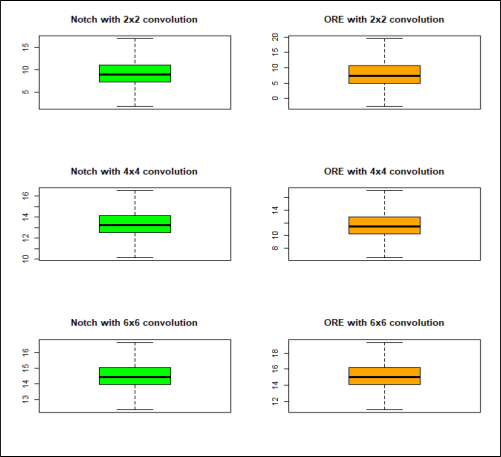
\includegraphics[width=\linewidth]{img/fig16-boxplot.png}
    \caption{Distribution of KL-Divergence for pairs of levels (n=10,000)}
    \label{fig:boxplot}
\end{figure}

When one looks at the previous statistics of the variability of the two generators, a
question may arise: Why does the mORE generator produce more varied levels for certain
feature sizes when compared to the Notch generator? The mORE generator is likely able to 
produce these more varied levels due to key differences between the generation approaches:
1) the Notch generator does not overlap its level segments, instead it attaches the by
their ends, 2) the mORE generator is able to work with a larger library of content than the
Notch generator, so it can explore more of the space of possible InfiniteTux levels.

To further illustrate point 1), a direct comparison between two levels generated by the
Notch and mORE generators is provided in \autoref{fig:overlap}. The top image shows a level
generated by mORE, and annotated with the unique chunks from the library as shown in \autoref{fig:more-chunks},
while the bottom shows a level generated by the Notch generator, with its chunks that were
previously described in \autoref{fig:ift-chunks}. Adjacent chunks in the first image are
regions of different colour, while a region that combines several chunks has several border
colours. Regions with alternating red and yellow borders are fairly linear, but regions
inculding magenta and green borders indicate three or four different chunks in the library
overalapping. There is an I-shaped region in the first image that is the result of an up-stair
and a down stair overlapping with a ground region. Regions such as these produce strange
features in the larger 6x6 features that KL-Divergence looks at, and they are not
guaranteed to appear. On the other hand, Notch levels are made of the same five or six chunks
with a degree of randomness to each chunk that varies smaller features within, such as hill
height, start, and end positions. Enemy and coin placement on top of these features creates
some variation, but still only two variants for these features are possible, a hill with or
without enemies. This may explain why there is more variation in larger-scale features in
mORE levels than Notch levels.

\begin{figure}[ht]
    \centering
    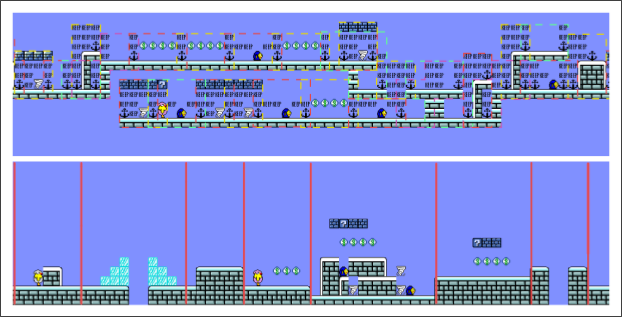
\includegraphics[width=\linewidth]{img/fig17-overlap.png}
    \caption{Comparison between two levels generated by mORE (top) and Notch (bottom)}
    \label{fig:overlap}
\end{figure}

To begin to compare the 2x2 features produced by each generator, it would be helpful to have
a visual aid. One is provided in \autoref{fig:top-forty}. The figure shows the most common
chunks of each generator at the top left, and the least common at the bottom right. In the
Notch level, air, plain ground, hill ground, and decorative tiles were the most common. For
mORE, air and various combinations of solid tiles were the most common. No decoration or
post-processing is done in mORE, so rounded corners are only present in the chunk library,
and appear less frequently. Several other features due not appear in mORE levels due to the 
lack of post-processing. This has an effect on the KL-Divergence metric. For each 2x2 feature
in two compared levels, KL-Divergence weighs the difference btween two levels higher if one
level has the feature and one does not than if both levels have the feature, but it occurs
more frequently in one compared to the other \cite{lucas2019}. This effect, combined with
combinations of chunks that mORE creates, is most likely responsible for much of the measured
difference between the genrated samples from both generators. It is also reasonable to expect
the variation of the mORE generator to grow if more chunks were added to the chunk library
it uses.

\begin{figure}[ht]
    \centering
    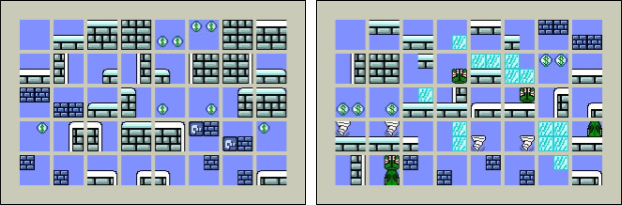
\includegraphics[width=\linewidth]{img/fig18-top40.png}
    \caption{40 most common features in a Notch (left) and mORE (right) level}
    \label{fig:top-forty}
\end{figure}

The final goal of the system was to provide a collaborative system for creating levels. Of
the described roles that a mixed-initiative system can take according to \cite{lawson1997},
the system most closely fits the collaborator and informer roles. The system collaborates with
the user by generating levels on command, or re-generating level sections as directed. By
making use of the chunk library that the user provides, it is able to accept input from the user.
It informs the user of errors regarding playability, component distribution, and the agent's
last playthrough, but it cannot correct the problems itself. As a collaborative system, it
would be more helpful to give the user more actionable feedback about their design than just
showing graphs that can be interpreted. However, thsi would likely require some kind of
background processing similar the existing A* agent. A more helpful suggestion to the user
would consider the library perhaps, and make recommendations to add chunk providing some 
missing mechanic. Perhaps the specific fixes could be provided bot the user instead of the
graphs, such as "There is a steep difficulty spike due to too many enemies in the area between
10 and 30", or "there is a large cluster of power-ups in the area from 10 to 20, consider
spreading them out". This type of feedback could provide better information to the user,
and would lighten the load on them by removing their need to interpret the graphs currently
displayed in the "Level Overview".